\chapter{Fundamentals}
\label{sec:fundamentals}

% \begin{itemize}
% 	\item describe methods and techniques that build the basis of your work
% 	\todo{don't get what methods and techniques i was using}
% 	\item include what's needed to understand your work (e.g., techniques, protocols, models, hardware, software, ...)
% 	\item exclude what's not (e.g., anything you yourself did, anything your reader can be expected to know, ...)
% 	\item review related work(!)
% 	\item recommended length: approximately one third of the thesis.
% \end{itemize}

In this chapter the fundamentals required for understanding the different approaches 
in this thesis using are explained.
This contains basic knowledge of the physical- and data link layer,
which are located in the first and second layer of the \ac{OSI} Model.
It also explains what types of transmissions exist.
In addition, the hardware used for this thesis is introduced.
The ESP-NOW protocol running on this hardware is also explained.
\todo{introduction in chapter Fundamentals ok?}

\begin{table}[h]
	\centering
	% \label{tab:layer_overview}
	\begin{tabular}{ |c| } 
		\hline
		Application layer\\
		\hline
		Presentation layer\\
		\hline
		Session layer\\
		\hline
		Network layer\\
		\hline
		\cellcolor{yellow!25}Data Link layer\\
		\hline
		\cellcolor{yellow!25}Physical layer\\
		\hline
	\end{tabular}
	\caption{\ac{OSI} model}
	\label{tab:OSI}
\end{table}

\section{IEEE 802.11 Specification Family}

The \ac{IEEE} 802 is a family of standards dealing with area networks different kinds.
\begin{itemize}
	\item 802.11 \ac{WLAN}
	\item 802.15.1 Wireless Personal Area Network (WPAN)
	\item 802.15.4 Low-rate WPAN (LR-WPAN)
	\item 802.16 Wireless metropolitan area network (WMAN)
\end{itemize}

For this thesis is the focus set to the 802.11, because of the accessability and wide functionality.
There are two \ac{BSS} defined:
\begin{itemize}
	\label{itm:bss}
	\item Infrastructure BSS\\
	A central element manages the network and all the traffic goes through. 
	Every \ac{STA} must always communicate via the \ac{AP} and never directly - exceptional: Direct Link Mode.
	An initial association must take place to use this \ac{BSS}.
	This is the most common mode a \ac{WLAN} is used.
	\item Independent BSS\\
	A network without a central station, where the network topology can flexible change over time.
	The communication happens directly between the Wireless Endsystems.
	Efficent routing can became a problem in more complex topologys.
\end{itemize}
The most common use in 802.11 is the Infrastructure mode, which is commonly used in office and home enviroments.\\ 

\subsection{Physical layer}

\todo{TOLJA: Was soll ich zum PHY alles sagen?}

In this thesis we sould take a breef look into the \ac{PHY} of the IEEE 802.11 standard, which is the first layer of the OSI model \ref{tab:OSI}.
This layer provides mechanical, electrical and other functional tools to activate or deactivate physical connections, maintain them and transmit bits over them. 
These can be, for example, electrical signals, optical signals (fiber optics, lasers) or electromagnetic waves (wireless networks).
There are several complements to the 802.11 standard, the most common are:

\begin{itemize}
	\item 802.11b \\
	supports larger bitrates with \ac{DSSS} or \ac{FHSS} as modulation from 1Mbit/s to 11Mbit/s.
	It uses the 2.4 GHz ISM band.
	\item 802.11a and 802.11g \\
	with \ac{OFDM} data rates are increased up to 54 Mbit/s.
	Where 802.11a is in the 5GHz ISM band 802.11g uses the 2.4GHz ISM band.
	\item 802.11n\\
	It also uses \ac{OFDM} and improves with additionaly \ac{MIMO}, channel bonding and frame aggregation to increase the bandwidth and decrease the overhead.
	Using 2.4 GHz and 5GHz ISM band.
	\item 802.11ac\\
	Support of wider channel and out of it higher bitrates. It also includes features like Multi-User MIMO.
	It only uses the 5 GHz ISM band.
	\item 802.11ax\\
	Like 802.11ac but with additional use of the 6GHz ISM band and better power control. 
	Also called WiFi6.
\end{itemize}

In this thesis the rather basic 802.11b is used with a transmission rate of 1Mbit/s.

\subsection{Data Link Layer}

The \ac{DL} Layer is the second lowest layer of the \ac{OSI} Model \ref{tab:OSI} and is split in two sublayers. 
The \ac{LLC} sublayer which multiplex protocols over the MAC layer while transmitting and to de-multiplex the protocols while receiving.
LLC provides the hop-to-hop flow and error control, allows multipoint communication over networks 
and it also adds frame sequence numbers.
But in this thesis we focus on the other data link sublayer.

The \ac{MAC} includes network protocols that regulate how multiple computers share the physical transmission medium they use. 
Without regulation, collisions and data loss would occur in the shared medium if several WES were to transmit simultaneously.
The \ac{MAC} Protocol Data Unit is additional added inside of the \ac{PHY} Payload. 
It contains the \ac{MAC} Header and encapsulated in it the \ac{MSDU}.

\begin{figure}[h]
	\centering
	\begin{bytefield}[bitwidth=1.1em, bitheight=\widthof{~Duration~}, boxformatting={\centering\small}]{29}
		\bitheader[endianness=little]{0-29} \\
		\bitbox{2}{FC} &
		\bitbox{2}{\rotatebox{90}{Duration}} &
		\bitbox{6}{Address\\1} &
		\bitbox{6}{Address\\2} &
		\bitbox{6}{Address\\3} &
		\bitbox{2}{SC} &
		\bitbox{6}{Address\\4}
	\end{bytefield}
	\caption{MAC header of a WLAN frame}
	\label{fig:mac_header}%
\end{figure}
\todo{Payload and FCS are missing}

\begin{itemize}
	\setlength\itemsep{-0.0em}
	\item \textbf{Frame Control Field:} Discribes the Type of frame:
	\begin{itemize}
		\setlength\itemsep{-0.5em}
		\item 00 Manegement Frame
		\item 01 Control Frame
		\item 10 Data Frame
	\end{itemize}
	\item \textbf{Duration:} Contains the \ac{NAV} value, specifies the transmission time required for the frame. 
	In order to save power to save energy, WES can defer access to the medium for this duration
	\item \textbf{Address fields:} Certain address fields are specified by the relative position of the address field.
	Not every address field is needed by certain frames. Each device is associated with a \ac{MAC} address.
	\begin{itemize}
		\setlength\itemsep{-0.0em}
		\item \ac{BSSID}
		\item Source Address
		\item Destination Address
		\item Transmitting STA Address
		\item Receiving STA Address
	\end{itemize}
	\item \textbf{Sequence Control:} Sequence number of the current frame modulo 4096.
	\item \textbf{MAC Payload:} The actual payload information of the \ac{MAC} layer. 
	The actual payload can differ, because the headers of the \ac{LLC} and ip etc. has to be subtracted.
	\item \textbf{Frame Check Frequence:} The sender calculates the checksum for the entire data block and appends it to the end of the block.
\end{itemize}

802.11ac and later using frame aggregation in order to reduce overhead.

\subsection{Carrier Sense Multiple Access/Collision Avoidance}

\ac{CSMA/CA} is composed of:
\begin{itemize}
	\setlength\itemsep{-0.0em}
	\item \textbf{CS (Carrier Sense):} Each station checks whether the medium is free before transmitting
	\item \textbf{MA (Multiple Access)}: Several stations share one medium, which can also be a cable.
	\item \textbf{CD (Collision Detection):} A schedule prevents two stations from starting their transmission at the same time.
\end{itemize}

\begin{figure}[h]
	\centering
	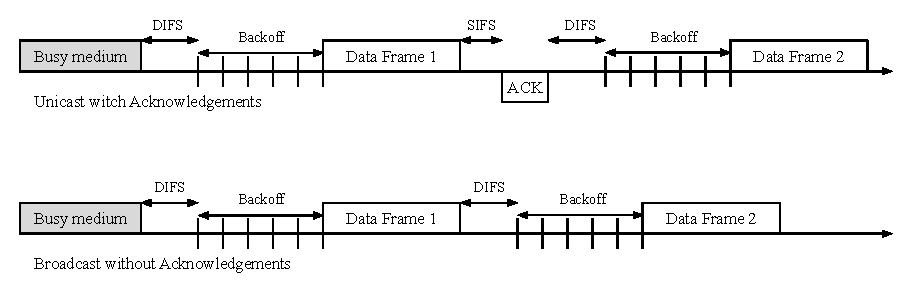
\includegraphics[scale=0.75]{figures/CSMA_CD.pdf}
	\caption{CSMA/CA with and without Acknolegements}
	\label{fig:CSMACD}
\end{figure}

Before a station transmitts data it has to check or listen to the medium to avoid collisiion resulting in packet loss.
Only when the medium is free, the station waits for a \ac{DIFS} and a random backoff.
The backoff is a random time within a \ac{CW} to prevent all stations from transmitting immediately after the \ac{DIFS}.
The \ac{CW} consists of several slots, each consisting of 20$\mu$s in 802.11b.
If a transmission was not successful, the station doubles the \ac{CW}, 
this doubles the average waiting time and is intended to prevent re-collisions.
The minimum \ac{CW} in 802.11b is set to 16 slots.

\subsection{Data Link Transmissions}

When packets are sent on the data link layer, they do not contain the headers to the layers above, such as TCP/IP.
Therefore, IP addresses cannot be used to transmit packets to another network.
There are three basic types of data link transmissions: unicast, broadcast and multicast.

\subsubsection*{Unicast}

The link layer unicast is used to send data over an single hop to the target \ac{WES} destination.
The link layer of each \ac{WES} checks the destination MAC address in the link layer header and 
discards the frame if the destination address does not match its own address.
It is therefore a direct communication between the transmitter and the WES.

Unicast is by default reliable.
When the Unicast reaches the destination \ac{WES} an acknowledgement frame is send back after the \ac{SIFS} + backoff.\todo{when to explain CSMA/DC?}
If the acknowledgement is not successfully received by the sender, the sender will repeat the transmission for a given number.
When the number is exceeded, the packet could not be delivered. 
If the number is set to zero, the unicast can be considered as non-reliable.
\TODO{example}

\begin{figure}[h]
	\centering
	\begin{tikzpicture}[node distance={15mm}, main/.style = {draw, circle}] 
		\node[main] (1) 				{TX}; 
		\node[main] (2) [right=0cm and 2cm of 1]	{$\text{RX}_1$}; 
		\node[main] (3) [above of =2]				{$\text{RX}_2$}; 
		\node[main] (4) [below of =2]				{$\text{RX}_3$}; 
		\draw[->] (1) -- (2);
	\end{tikzpicture} 
	\caption{Unicast Transmission}
	\label{fig:unicast_topology}
\end{figure}

\subsubsection*{Broadcast}

If a packet should be received from all \ac{WES}'s it can be distributed as broadcast.
The \ac{MAC} address of the destination address in the link layer is set to the common broadcast address, which is ff:ff:ff:ff:ff:ff.\\
In contrast to unicast, broadcast is not reliable. 
This is mainly because the packet is addressed to all nodes at the same time, and if link layer acknoledgements would be used, 
the acknoledgements would be sent by all nodes at the same time, 
because there is no mechanism in which order acknoledges should be answered. 
In addition, the sender of a broadcast does not know how many WESs he is addressing the packet to in the first place.
Retransmitting acknoledgements would lead to massive collision and loss of acknoledgements.
E.g. management information in a \ac{WLAN} is sent in a broadcast mode, because it has to reach every \ac{WES} and isn't worth to be acknoleged.

\begin{figure}[h]
	\centering
	\begin{tikzpicture}[node distance={15mm}, main/.style = {draw, circle}] 
		\node[main] (1) 				{TX}; 
		\node[main] (2) [right=0cm and 2cm of 1]	{$\text{RX}_1$}; 
		\node[main] (3) [above of =2]				{$\text{RX}_2$}; 
		\node[main] (4) [below of =2]				{$\text{RX}_3$}; 
		\draw[->] (1) -- (2);
		\draw[->] (1) -- (3);
		\draw[->] (1) -- (4);
	\end{tikzpicture} 
	\caption{Unicast Transmission}
	\label{fig:unicast_topology}
\end{figure}

\subsubsection*{Multicast}

\TODO{Mutlicast explain multicast mac address}
When the same packet should be transmitted to multiple \ac{WES}'s, but not to all, multicast can be used.
Transmitting the same packet multiple times via unicast is wasteful.
There are different approaches to realize acknowledgements for mutlicasts, they differ mainly by the respective field of application.
\TODO{examples for multicast ack + related work}
Level 2 multicast is often used for large files in audio or video streams, where a big amount of data is distributed and multiple clients listen simultaneously.

\begin{figure}[h]
	\centering
	\begin{tikzpicture}[node distance={15mm}, main/.style = {draw, circle}] 
		\node[main] (1) 				{TX}; 
		\node[main] (2) [right=0cm and 2cm of 1]	{$\text{RX}_1$}; 
		\node[main] (3) [above of =2]				{$\text{RX}_2$}; 
		\node[main] (4) [below of =2]				{$\text{RX}_3$}; 
		\draw[->] (1) -- (2);
		\draw[->] (1) -- (4);
	\end{tikzpicture} 
	\caption{Unicast Transmission}
	\label{fig:unicast_topology}
\end{figure}
\todo{complete figure MC}


\section{Light protocols}

There are several lighting protocols that are used. The field of application ranges from wired CAN buses over ethernet cables to wireless WLAN networks.
To give a short insight, some of the most important protocols are explained below.

\subsection{DMX-512A}
\ac{DMX} 512A, is the current industry standard for stage lighting. It is based on \ac{CANproto}, therefore it uses wires.
Physically is the DMX protocol transmitted over a differential pair of lines using the RS-485 voltage levels. 
The bus signal is updated with 44Hz.
According to the specification are XLR-5 type connectors are to be used. \todo{image der connectoren}

\TODO{Show Hardware e.g. DMX Plug}

The endsystems are called fixture because it's most likely a lighting installation which is mounted somewhere, 
this could be a moving-head, fresnel, spotlight, stroboscope or any other light installation.
It could also be a fog machine that emits fog on an appropriate signal.

All devices are daisy chained together visualized in \ref{fig:dmx_diagram}.
The DMX controller is in the begin of each chain.
The receiving endsystems, are chained behind each other from output to input. 
A terminator, specified in the DMX specification, is to be connected to the final output.
 
\begin{figure}[h]
	\centering
	\begin{tikzpicture}[thick,
	    TFblock/.style= {
	        draw,  
	        minimum size=1.5cm}]
	
		% Blocks
		\node [TFblock,fill=green!10] (a) {\footnotesize{\ \ \ \ \ \ \ \ OUT}};
		\node [TFblock,fill=white!20,] (b) [right= of a] {\footnotesize{IN\ \ \ \ \ OUT}};
		\node [TFblock,fill=white!20] (c) [right =of b] {\footnotesize{IN\ \ \ \ \ OUT}};
		\node [TFblock,fill=orange!10] (d)[right =of c] {\footnotesize{IN\ \ \ \ \ \ \ \ \ \ \ \ }};

		% % Arrows
		\draw[-latex] 
		    (a.east) edge (b.west)
		    (b.east) edge (c.west)
		    (c.east) edge (d.west) ;

		% Labels
		\node[below=0.8cm] at (a){Controller};
		\node[below=0.8cm] at (b){Fixture 1};
		\node[below=0.8cm] at (c){Fixture n};
		\node[below=0.8cm] at (d){Terminator};
		\node[above=0.2cm] at (barycentric cs:b=1,c=1){ ... };

	\end{tikzpicture}
	\caption{Block Diagram of an DMX Universe}
	\label{fig:dmx_diagram}
\end{figure}

The hole chain is called DMX-Universe and can contain a set of 512 channel.
If there is a need of more channels one needs more DMX universes - each channel consists of one byte.
Due to the fact that a DMX universe always has its own bus, starting from a new controller can lead to inconveniences.

A channel in the event technology is to distinguish between e.g. a WiFi channel.
Each endsystem is assigned at least one, but usually several channels.
Every endsystems knows which channel is intended for it, this must to be preset.

For example: An RGB-LED spotlight could have three channels, one for each color.
Due to the resolution of one byte, the individual colors can (theoretically) be controlled in 256 different intensities.
If the Channel 0-56 are already used, it could be set to channel 57, 58, 59.
Any other free channel range would also be possible, provided it is connected.
There exist hardware with automatic-address-assignment.

\TODO{Image of fixtures distributed on channel}

Since \ac{DMX} is unidirectional it can be assumed that the endsystems generally only receive or forward (daisy chain) control signals sent from the control console.
This is a major limitation of DMX, beside of the rather small universe size.
It is also not reliable, the use of fire installations is therefore considered too dangerous.

\subsection{Art-Net}
\label{sec:artnet}
\begin{itemize}
	\item Example of an wifi protocol
	\item 2.4 or 5GHz
	\item DMX-Like
	\item related work
\end{itemize}

Due the limitation of 512 channel for each universe there where protocols implemented using the 
Art-Net also called Art-Net DMX is 

\section{ESP Platform}

Almost every 802.11 capable \ac{MCU} could be picked for this research.
But there are several reasons why the ESP Platform from Espressif is a valid choice.
There are several chips provided by Espressif with WiFi specifications, these chips are very affordable (\todo{TOLJA: ESP32 Kosten in € 2021 aufführen? Link? Datum?}) 
and althrough the ongoing chip crysis (2021) there are easy to get, in contrast of the also very popular Chips from the manufacturer Arduino, which are also more expansive.
Espressif supports an own development IDF to flash the chips, with minor tweeks it's also to use the Arduino IDE.\\
However the properitary protocol ESP-Now which, just supported in the ESP Ecosystem, is discussed below \cref{sub:ESP-Now} 
and has promising properties for a solid and fast realisation of a low level protocol.
\TODO{paper about esp above arduino}

\subsection{ESP32 Hardware}

The chip ESP32 is quite common in DIY projects around everything from home automation to light installations 
and can baught on development boards, which are ready to use.
The chip \ref{fig:esp32} is promoted with several features: \todo{this is cited from: link zum esp32 datasheet}
\begin{itemize}
	\setlength\itemsep{-0.0em}
	\item Fast CPU (2 cores at 240 MHz)
	\item 802.11 b/g/n with up to 150 Mbps (2.4GHz)
	\item Wifi Multimedia (WMM)
	\item Immediate Block ACK
	\item Automatic Beacon monitoring (hardware TSF)
	\item Virtual Wi-Fi Interfaces
	\item Simultaneous support for Infrastructure, SoftAP, and Promiscuous modes
	\item Bluetooth v4.2 BR/EDR and Bluetooth LE
	\item Advanced Peripheral Interfaces: GPIO, ADC, DAC, touch sensors, hall sensor, 
	SPI, I2S, I2C, UART, CAN, RMT (TX/RX), Motor/LED PWM 
\end{itemize}

\begin{figure}[h]
	\centering
	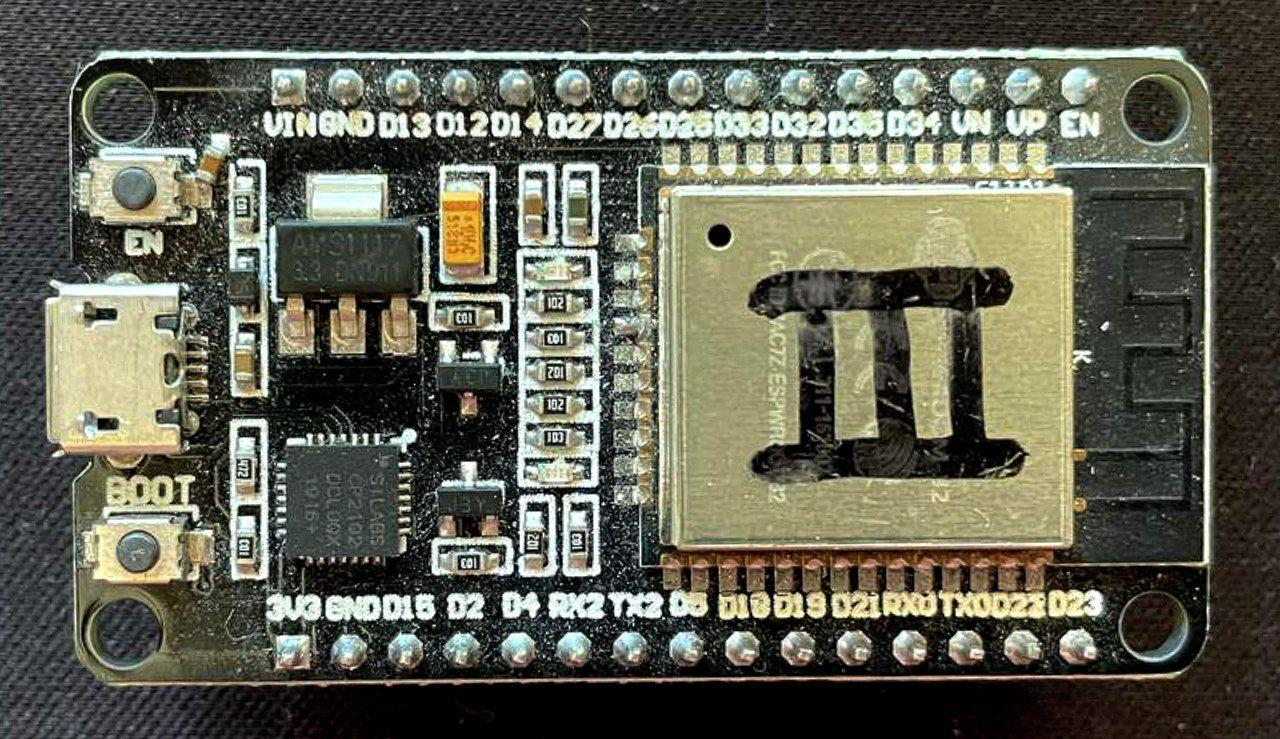
\includegraphics[scale=0.2]{figures/espdevboard.jpg}
	\caption{ESP32 Devboard (Devkit V1)}
	\label{fig:esp32}%
\end{figure}

\TODO{final words to the ESP32 Hardware - a lot of features for a cheap hardware}

\subsection{ESP-Now}
\label{sub:espnow}
ESP-NOW is a properitary protocol developed by Espressif. 
ESP-NOW is widely used in smart light, remote controlling, sensor, etc\todo{cite ESP documentation website}. 
It is a conectionless protocol, so the \ac{WES}'s are in Ad-Hoc mode insted of \ac{STA}.
It is just supported on the ESP8266, ESP32 and ESP32s, all chipsets from Espressif, but they are compatible with each other.
Because of this, a ESP-Chip as gateway is needed to interact from the outside to the ESP-NOW communication. 

Through the hardware limitation of the boards it can just be used on the 2.4 GHz frequncy band.
ESP-NOW allows 10 ESPs for pairing with encryption and up to 20 without encryption.
Espressif promises throuput of up to 30MBit/s with and a possible range of up to 1km.
However \emph{\textcite{ESPNOWPaper}} measured a range of the unmodified onboard antenna of the ESP32 
and just got a \emph{\textcite{ESPNOWPaper} stable commication up to 190m in open field}.\\

The focus of the ESP-NOW protocol is on low power consumption.
A connectionless communication between \ac{WES}'s not only saves energy during the authentication process, 
Additionally, is the commonication the the properties of the ad-hoc mode, direct and not over a second access point.
The protocol has a limitation of a limeted payload of 250 byte for each transmission.
It also has a much less overhead, which results in shorter airtime, less disturbances and also less power consumption through the antenna 
(latter is not relevant for this thesis).
There is no TCP/IP header to be transmited. 
For very small payloads, this offset can become dispropotional.

The default ESP-NOW bit rate is 1 Mbps it uses a channelwidth of 20MHz, there is no double channel (40Mbit/s or higher) used.
But e.g. the low energy, high range protocol Long Range Wide Area Network (LoRaWAN) suffers from a to slow throuput for this application.

To undersant what ESP-NOW does it needs to take a look to the vendor-specific action frame transmiting ESP-NOW data. 
\todo{cite somehow the ESP-NOW documentation pdf: ESP-IDF Programming Guide: ESP-NOW, source: \url{https://docs.espressif.com/projects/esp-idf/en/latest/esp32/api-reference/network/esp_now.html}}
\TODO{Explain Vendor Specific Frames!}

% \url{https://www.heise.de/tipps-tricks/}

visualized in \ref{fig:esp-now_frame_format}.

\begin{table}[h]
	\centering
	\begin{tblr}{	hlines,
					vlines,
					rows = {ht=1.3cm},
					columns = {halign=c},
					colspec = {XXXXXX},} 
	\makecell{MAC\\Header} & \makecell{Category\\Code} & \makecell{Org.} & 
	\makecell{Random\\Values} & \makecell{Vendor\\Specific\\Content} & \makecell{FCS}\\
	\end{tblr}
	\begin{tabularx}{\linewidth}{ X X X X X X }
		\makecell{\footnotesize{24}} & \makecell{\footnotesize{1}} & \makecell{\footnotesize{3}} & 
		\makecell{\footnotesize{4}} & \makecell{\footnotesize{7 $\sim$ 255}} & \makecell{\footnotesize{4}} \\
	\end{tabularx}
	\caption{ESP-NOW Frame Format}
	\label{fig:esp-now_frame_format}
\end{table}

\begin{itemize}
	\setlength\itemsep{-0.0em}
	\item \textbf{MAC Header:} As ESP-NOW is connectionless, the MAC header differs from that of standard frames.
	\item \textbf{Category Code:} The Category Code field is set to the value(127) indicating the vendor-specific category.
	\item \textbf{Organization Identifier:} The Organization Identifier contains a unique identifier (0x18fe34), which is the first three bytes of MAC address applied by Espressif.
	\item \textbf{Random Value:} The Random Value filed is used to prevents relay attacks.
	\item \textbf{Vendor Specific Content:} The Vendor Specific Content contains vendor-specific fields (table \ref{fig:esp_now_vendor_format})
	\item \textbf{Frame Check Sequence:} Used for error correction in layer 2.
\end{itemize}

Inside of the ESP-NOW frame \ref{fig:esp-now_frame_format} is the vendor specific content visualized in \ref{fig:esp_now_vendor_format}. 

\begin{table}[h]
	\begin{tblr}{	hlines,
					vlines,
					rows = {ht=1.3cm},
					columns = {halign=c},
					colspec = {XXXXXX},} 
		\makecell{Element\\ID}& \makecell{Length} & \makecell{Org.\\Identifier} & \makecell{Type} & \makecell{Version} & \makecell{Body}  \\
	\end{tblr}
	\begin{tabularx}{\linewidth}{ X X X X X X }
		\makecell{\footnotesize{1}} & \makecell{\footnotesize{1}} & \makecell{\footnotesize{3}} & \makecell{\footnotesize{1}} & \makecell{\footnotesize{4}} & \makecell{\footnotesize{7 $\sim$ 250}} \\
	\end{tabularx}

	\caption{Vendor Specific Action Frame}
	\label{fig:esp_now_vendor_format}
\end{table} 

\begin{itemize}
	\setlength\itemsep{-0.0em}
	\item \textbf{Element ID:} The Element ID field is set to the value (221), indicating the vendor-specific element.
	\item \textbf{Length:} The length is the total length of Organization Identifier, Type, Version and Body.
	\item \textbf{Organization Identifier:} The Organization Identifier contains a unique identifier(0x18fe34), which is the first three bytes of MAC address applied by Espressif.
	\item \textbf{Type:} The Type field is set to the value (4) indicating ESP-NOW.
	\item \textbf{Version:} The Version field is set to the version of ESP-NOW.
	\item \textbf{Body:} The Body contains the ESP-NOW data.
	\todo{this is cited from espressif manual!!}
\end{itemize}

It is worth to mention, that the vendor specific content \ref{fig:esp-now_frame_format} is allowed to contain up to 255 byte,
but the sum over all values in \ref{fig:esp_now_vendor_format} if the body would contain the maximum of 250 bytes, 
leads to a total of 260 bytes.\todo{255 != 250 is it really that important?}
The values are from the documentation of ESP-NOW from Espressif.
They also claim, that broadcast is not supported in ESP-NOW, but it is.
It seems that the documentation isn't complitly finished (or translated).

\subsection{ESP-Now vs Art-Net Baseline}
\todo{subsection can be on a wrong position!}
\TODO{remove newpage command}
\begin{itemize}
	\item Network stack diagram
	\item baseline
\end{itemize}

\TODO{ESP-NOW Baseline Artnet should be moved to Design part??}